\documentclass[../TDON2_inter.tex]{subfiles}%

\begin{document}
\section[s]"1"{Mesure de la vitesse du son avec des trous d'\textsc{Young}}

\enonce{%
	On considère un dispositif composé de deux trous d'\textsc{Young} percés dans un
	écran opaque et séparés d'une distance $a = \SI{10.0}{cm}$. Une onde ultrasonore
	de fréquence $f = \SI{40}{kHz}$ est envoyée en direction des trous. L'amplitude
	de l'onde en sortie des trous est mesurée en utilisant un récepteur qui peut
	être translaté suivant un axe (O$x$) parallèle à la direction des trous et situé
	à une distance $D = \SI{50.0}{cm}$ du plan des trous. Le dispositif expérimental
	est représenté sur la figure 1. Par la suite, les valeurs de $D$ et $a$ sont
	supposées connues avec une précision de \SI{1}{mm} et l'incertitude-type sur la
	valeur de $f$ est supposée négligeable.

	\begin{center}
		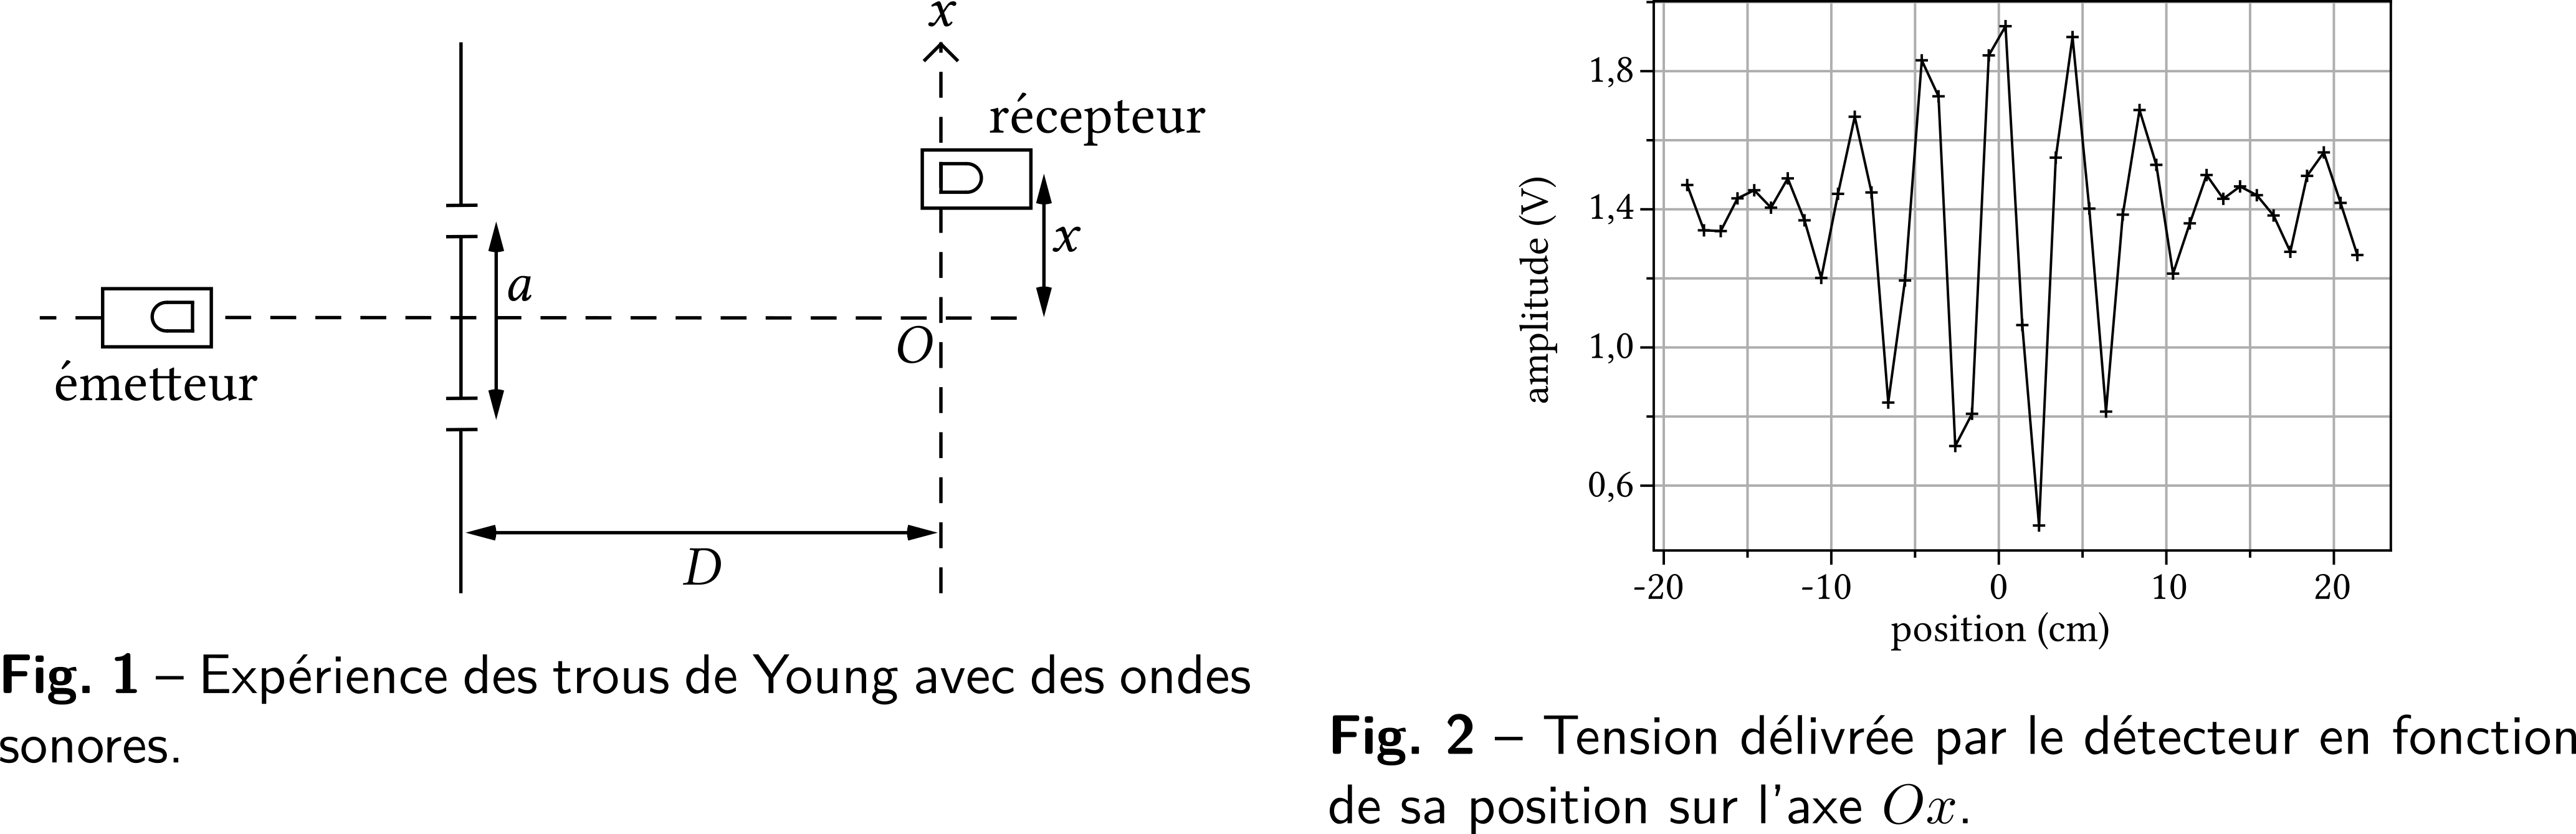
\includegraphics[width=\linewidth]{young_son-plain}
	\end{center}
}

\QR{%
	En supposant que la condition $D \gg a,\,\,x$ est vérifiée, donner
	l'expression de l'interfrange $i$ correspondant à la distance sur l'axe
	(O$x$) entre deux interférences constructives.
}{%
	L'interfrange dans une expérience de trous d'\textsc{Young} dont les
	fentes sont séparées de $a$ est
	\[\boxed{i = \frac{\lambda D}{a}}\]
}

\enonce{%
	Le résultat de la mesure de l'amplitude du signal électrique délivré par le
	récepteur en différentes positions sur l'axe (O$x$) est représenté sur la figure
	2.
}

\QR{%
	À partir de la figure 2, estimer la valeur de l'interfrange ainsi que
	son incertitude-type.
}{%
	On mesure avec une règle graduée au millimètre pour mesurer
	(conversion d'échelle comprise) $4i = \SI{17.1}{cm}$. La précision
	est ici limitée par l'écart entre deux positions de mesure du
	détecteur. Avec l'échelle de la figure et le facteur $1/\sqrt{3}$, on
	trouve l'incertitude-type de mesure $u_{4i} = \SI{0.8}{cm}$. Ainsi,
	\[\boxed{i = \SI{4.3\pm0.2}{cm}}\]
}

\QR{%
En déduire une estimation de la célérité $c$ du son dans l'air ainsi que de
son incertitude-type. On néglige toute incertitude sur la fréquence $f$. On
rappelle la formule de propagation des incertitudes~:
\[
	y = a x_1{}^{\alpha_1}x_2{}^{\alpha_2}
	\Ra
	\sqrt{%
		\pa{\alpha_1 \frac{u (x_1)}{x_1}}^2 +
		\pa{\alpha_2 \frac{u (x_2)}{x_2}}^2
	}
\]
}{%
En utilisant l'expression de l'interfrange et de $\lambda = c/f$, on a
\[
	c = \lambda f = \frac{fa}{D}
	\Lra
	c = \SI{3.4e2}{m.s^{-1}}
\]
On détermine d'abord l'incertitude sur $\lambda = \frac{\lambda D}{a}$ avec la
formule de propagation, puis $u(c) = f \cdot u(\lambda)$~:
\begin{gather*}
	\frac{u(\lambda)}{\lambda}
	= \sqrt{\left(\frac{u(i)}{i}\right)^2 +
		\left(\frac{u(a)}{a}\right)^2 +
		\left(\frac{u(D)}{D}\right)^2}
	\qavec
	\left\{
	\begin{array}{rcl}
		\lambda & = & \SI{8.4}{mm}                               \\
		i       & = & \SI{4.3}{cm}                               \\
		u(i)    & = & \SI{0.2}{cm}                               \\
		a       & = & \SI{10.0}{cm}                              \\
		u(a)    & = & \frac{\SI{1}{mm}}{\sqrt{3}} = \SI{0.6}{mm} \\
		D       & = & \SI{50.0}{cm}                              \\
		u(D)    & = & \frac{\SI{1}{mm}}{\sqrt{3}} = \SI{0.6}{mm}
	\end{array}
	\right.\\
	\mathrm{A.N.~:}\quad
	\boxed{c = \SI{3.4\pm0.1e2}{m.s^{-1}}}
\end{gather*}
}

\enonce{%
	Un phénomène de diffraction est observé lorsqu'une onde traverse un trou de
	rayon $r \approx \lambda$. Le faisceau en sortie du trou présente alors un
	demi-angle d'ouverture $\theta$ tel que $\sin(\theta) \approx \lambda/2r$.
}

\QR{%
	À partir de la figure 2, estimer l'ordre de grandeur du rayon des
	trous utilisés dans l'expérience.
}{%
	La diminution de l'amplitude des interférences lorsque $x$ augmente
	est due au phénomène de diffraction par un trou d'\textsc{Young}. Sur la
	figure 2, on peut voir que l'amplitude des interférences s'annule pour
	$x_a \approx \SI{15}{cm}$. Or, d'après la figure 1, $\tan(\theta) =
		x_a/D$~; ainsi, en combinant avec $\sin(\theta) \approx \lambda/2r$ et
	avec l'approximation des petits angles ($\tan(\theta) \approx \theta$ et
	$\sin(\theta) \approx \theta$), on a
	\[
		\frac{x_a}{D} \approx \frac{\lambda}{2r}
		\Lra
		\boxed{r \approx \frac{\lambda D}{2x_a} \approx \SI{1.4}{cm}}
	\]
}

\end{document}
